% Created 2025-03-06 Thu 18:44
% Intended LaTeX compiler: pdflatex
\documentclass[11pt]{article}
\usepackage[utf8]{inputenc}
\usepackage[T1]{fontenc}
\usepackage{graphicx}
\usepackage{longtable}
\usepackage{wrapfig}
\usepackage{rotating}
\usepackage[normalem]{ulem}
\usepackage{amsmath}
\usepackage{amssymb}
\usepackage{capt-of}
\usepackage{hyperref}
\usepackage{minted}
\usepackage[margin=0.5in]{geometry}
\hypersetup{colorlinks, linkcolor=black}
\usepackage{geometry}
\geometry{top=2cm}
\geometry{bottom=2cm}
\usepackage{fancyhdr}
\pagestyle{fancy}
\fancyhf[L]{Redes de área local}
\fancyhf[R]{Tema 04 - Cableado estructurado}
\fancyfoot[R]{ismaelmacarenochouikh1@gmail.com}
\fancyfoot[L]{CC BY-NC-SA 4.0}
\usepackage{parskip}
\usepackage{mdframed}
\usepackage{fancyvrb}
\usepackage{xcolor}
\definecolor{shadecolor}{RGB}{220,220,220}
\newenvironment{shadedcode}{%
\VerbatimEnvironment
\begin{mdframed}[backgroundcolor=shadecolor,linewidth=0pt]}%
{\end{mdframed}}
\usepackage{attachfile2}
\newcommand{\textattachfilecolor}[2]{\textattachfile[color=0 0 0.5]{#1}{\textcolor{blue}{#2}}}
\usepackage[spanish]{babel}
\usepackage{datetime2}
\DTMlangsetup[es-ES]{ord=raise}
\renewcommand{\dateseparator}{/}
\usepackage{titlesec}
\usepackage{afterpage}
\newcommand\blankpage{\null\thispagestyle{empty}\newpage}
\usepackage{colortbl}
\usepackage{pdfpages}
\usepackage{tcolorbox}
\usepackage{listings}
\usepackage[spanish]{babel}
\lstset{
inputencoding=utf8,
extendedchars=true,
literate={ñ}{{\~n}}1 {Ñ}{{\~N}}1 {á}{{\'a}}1 {é}{{\'e}}1 {í}{{\'i}}1 {ó}{{\'o}}1 {ú}{{\'u}}1 {Á}{{\'A}}1 {É}{{\'E}}1 {Í}{{\'I}}1 {Ó}{{\'O}}1 {Ú}{{\'U}}1,
basicstyle=\ttfamily,
breaklines=true,
columns=fullflexible,
keepspaces=true,
language=TeX,
morekeywords={*, -, **, /}
}
\author{Ismael Macareno Chouikh}
\date{\today}
\title{Tema 04 - Cableado Estructurado}
\hypersetup{
 pdfauthor={Ismael Macareno Chouikh},
 pdftitle={Tema 04 - Cableado Estructurado},
 pdfkeywords={},
 pdfsubject={},
 pdfcreator={Emacs 29.4 (Org mode 9.6.15)}, 
 pdflang={Spanish}}
\begin{document}

\maketitle
\tableofcontents

\blankpage

\section{Definiciones de cableado estructurado}
\label{sec:orgb986b21}
\subsection{Definición I}
\label{sec:org7222b1d}
El \textbf{cableado estructurado} es la técnica que permite
\begin{itemize}
\item cambiar
\item identificar
\item mover
\end{itemize}
periféricos o equipos de una red con flexibilidad y sencillez.
\subsection{Definición II}
\label{sec:org125738b}
Sistema colectivo de:
\begin{itemize}
\item cables
\item canalizaciones
\item conectores
\item etiquetas
\item espacios
\end{itemize}
y demás dispositivos que deben ser instalados para establecer una infraestructura de telecomunicaciones genérica en un edificio o campus
\subsection{Definición III}
\label{sec:org0055c92}
Distribución de cables en un edificio que comprenda las necesidades de comunicación actuales y futuras.

\section{Características}
\label{sec:org6728703}
\begin{itemize}
\item Toda solución de cableado estructurado debe ser modular.
\item Comprende la transmisión de voz y datos
\item Los equipos de interconexión de los módulos se sitúan en lugares centralizados, facilitando la detección de problemas de cableado y su solución sin afectar al resto de la red.
\end{itemize}

\section{Normativa}
\label{sec:org3499029}
Las normas más importantes a saber son:
\begin{itemize}
\item EIA/TIA 568 y otras
\item ISO/IEC 11801
\item EN 50173
\end{itemize}

\subsection{Estándar ANSI/TIA/EIA-568-A}
\label{sec:org8446c8b}
Estándar ANSI/TIA/EIA-568-A de Cableado de Telecomunicaciones para Edificios Comerciales. El propósito de esta norma es permitir la planificación e instalación de cableado de edificios
con muy poco conocimiento de los productos de telecomunicaciones que serán instalados con posterioridad.

\subsection{Complemento de la norma 568-A en aspectos de cableado}
\label{sec:orgd32fd96}
\begin{itemize}
\item \textbf{Estándar ANSI/TIA/EIA-569-A}: de Rutas y Espacios de Telecomunicaciones para Edificios Comerciales.
\item \textbf{EIA/TIA 570}: establece el cableado de uso residencial y de pequeños negocios.
\item \textbf{Estándar ANSI/TIA/EIA-606}: Administración para la Infraestructura de Telecomunicaciones de Edificios Comerciales.
\item \textbf{EIA/TIA 607}: define al sistema de tierra física y el de alimentación bajo las cuales se deberán de operar y proteger los elementos del sistema estructurado.
\end{itemize}

\section{Ventajas}
\label{sec:org7d5aa9a}
\begin{itemize}
\item independiente de la aplicación y del proveedor
\item puede conectarse en cualquier punto del edificio y trabajar del mismo modo
\item crecimiento de la red sin añadir excesiva complejidad a la misma
\item Los problemas que pudieran surgir quedan aislados en el módulo correspondiente.
\end{itemize}

\section{Subsistemas}
\label{sec:orge5772fb}
\begin{itemize}
\item \emph{backbone} o subsistema troncal
\item subsistema horizontal
\item subsistema administrativo (conecta el vertical con el horizontal)
\item subsistema de puesto de trabajo (\emph{patch cord})
\item subsistema de campus (instalaciones grandes o multi-edificio)
\item Otros:
\begin{itemize}
\item instalación de entrada
\item sala de equipos
\end{itemize}
\end{itemize}



\section{Ejemplo práctico}
\label{sec:orgbceb9b0}
\begin{center}
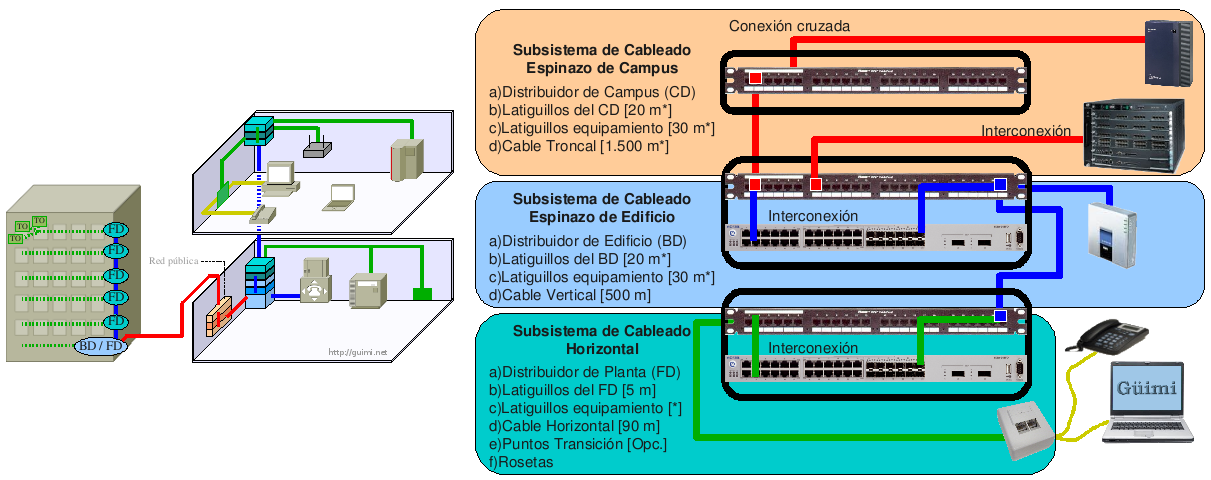
\includegraphics[width=.9\linewidth]{./media/ejemplo-cableado1.png}
\end{center}

\section{Subsistemas troncal y horizontal}
\label{sec:org8544716}
\subsection{Subsistema troncal o \emph{backbone}}
\label{sec:org85a8878}
\begin{itemize}
\item Proporciona interconexión entre la sala de equipos, subsistemas administrativos e instalaciones de entrada.
\item Necesita tener gran ancho de banda
\begin{itemize}
\item implica cableado de alta velocidad
\end{itemize}
\end{itemize}
\subsection{Subsistema horizontal}
\label{sec:org86bc51e}
\begin{itemize}
\item Cableado e interconexión entre elsubsistema administrativo y el área de trabajo.
\item Necesita menor ancho de banda que el vertical.
\end{itemize}

\section{Subsistemas administrativo y de trabajo}
\label{sec:org64edf50}
\subsection{Subsistema administrativo}
\label{sec:orge659e67}
\begin{itemize}
\item Conexiones entre subsistemas vertical y horizontal
\item Compatibiliza la transmisión vertical y la horizontal en caso de que se necesite
\end{itemize}
\subsection{Subsistema o área de trabajo}
\label{sec:org48b8223}
\begin{itemize}
\item Conecta el horizontal con el equipo de usuario
\item Roseta y cable directo al PC y/o teléfono
\end{itemize}

\section{Otros elementos}
\label{sec:org38f8c7e}
\subsection{Instalación de entrada o acometida}
\label{sec:orgd8eac87}
\begin{itemize}
\item Es el punto donde la instalación exterior se conecta al edificio.
\item Este punto puede estar utilizado por servicios de redes públicas, redes privadas del cliente, o ambas.
\item Separa ámbitos público y privado.
\end{itemize}
\subsection{Sala de equipos}
\label{sec:orgcccd9e0}
\begin{itemize}
\item Espacio centralizado para todo tipo de servidores y equipos de comunicaciones comunes a todo el edificio.
\end{itemize}

\section{Elementos del cableado estructurado}
\label{sec:orgb28bddb}
\subsection{Cables}
\label{sec:orgad77743}
\begin{itemize}
\item UTP para el subsistema horizontal y \emph{patch cords}.
\item Fibra, coaxial o UTP/STP de alta velocidad para el subsistema vertical.
\end{itemize}
\subsection{Conectores - I}
\label{sec:org5c97213}
\begin{itemize}
\item RJ45 para datos
\end{itemize}
\begin{center}
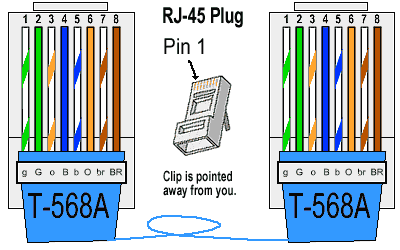
\includegraphics[width=.9\linewidth]{./media/RJ45-Pinout.png}
\end{center}
\subsection{Conectores - II}
\label{sec:orgc7ee4e3}
\begin{itemize}
\item RJ11 para voz
\end{itemize}
\begin{center}
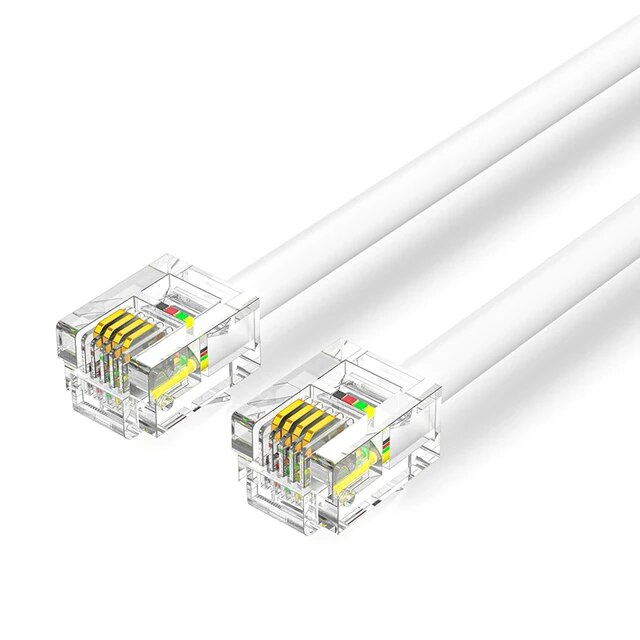
\includegraphics[width=.9\linewidth]{./media/cable-de-telefono-rj11-6p4c-m-m-3-m-blanco.png}
\end{center}
\subsection{Rosetas o tomas de usuario}
\label{sec:org81956bf}
\begin{itemize}
\item Elementos donde se conectan los \emph{patch cord} de las áreas de usuario
\end{itemize}
\begin{center}
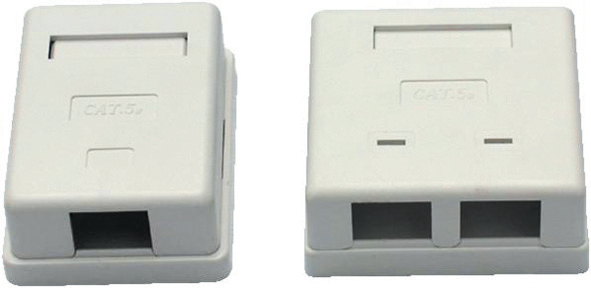
\includegraphics[width=.9\linewidth]{./media/ethernet_es-roseta-vacia.png}
\end{center}
\subsection{Paneles de parcheo}
\label{sec:orge8df113}
\begin{itemize}
\item Elementos de terminación de una conexión. Facilitan conectar, interconectar y reconectar elementos en la red. Se instalan en los \emph{racks}.
\end{itemize}
\begin{center}
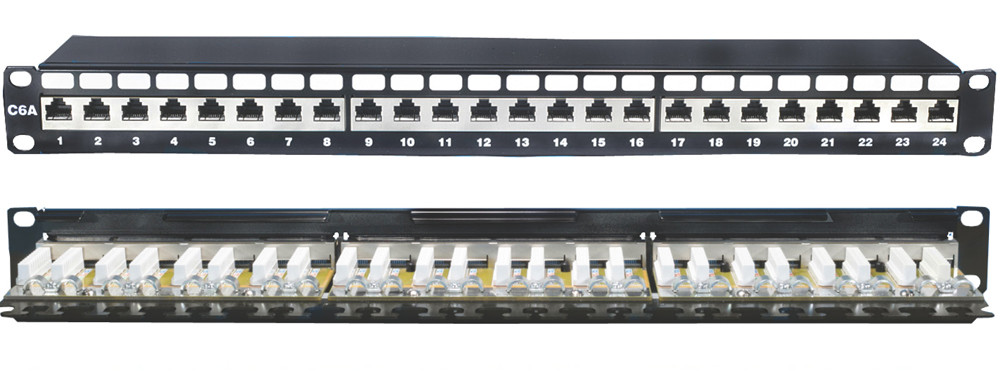
\includegraphics[width=.9\linewidth]{./media/667233583716241408.png}
\end{center}
\subsection{Canaletas y falsos suelos}
\label{sec:org9151fae}
\begin{itemize}
\item Para ocultar el cableado
\end{itemize}
\begin{center}
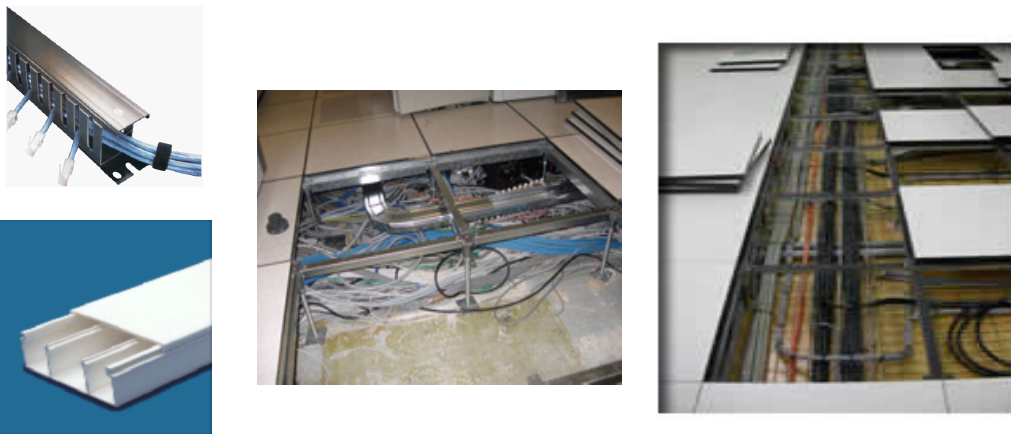
\includegraphics[width=.9\linewidth]{./media/canaleta-falsoSuelo.png}
\end{center}
\subsection{Armarios de comunicación}
\label{sec:orgd9edaae}
\begin{itemize}
\item Albergan paneles de parcheo, \emph{switches}, \emph{hubs} y el cableado de interconexión.
\end{itemize}
\begin{center}
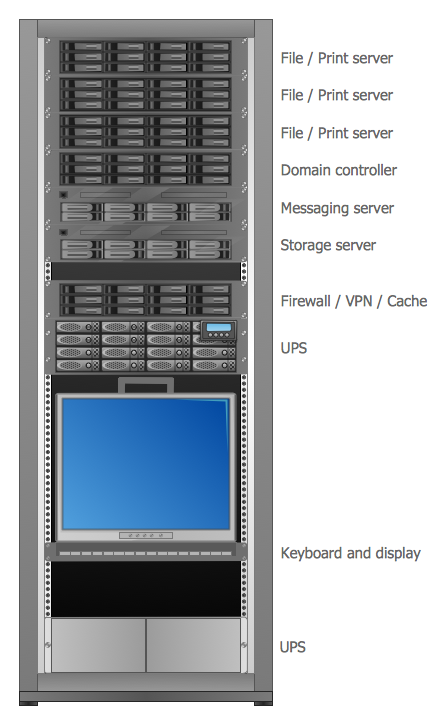
\includegraphics[width=.9\linewidth]{./media/COMPUTERS-AND-NETWORKS-Rack-diagrams-Typical-Server-Rack-Diagram.png}
\end{center}

\section{Recomendaciones en la instalación}
\label{sec:org61b90c0}
\subsection{Subsistema horizontal}
\label{sec:org8a4f705}
\begin{itemize}
\item Definir previamente la cantidad de puestos por planta.
\begin{itemize}
\item Calcular 1 puesto de trabajo por cada 10m2 aproximadamente
\end{itemize}
\item Definir cuántas conexiones RJ45 y RJ11 se necesitan por puesto de trabajo
\begin{itemize}
\item Normalmente por puesto 2, una para datos y otra para voz
\end{itemize}
\item Definir tipos de canalizaciones y rosetas que se requieren
\item Definir la mejor ubicación de los armarios
\item Definir la cantidad de cable que se necesita, sabiendo las limitaciones de longitud especificadas para ese cable
\item Prever un 15 o 20\% de conexiones libres
\end{itemize}
\subsection{Subsistema vertical}
\label{sec:org0671738}
\begin{itemize}
\item Definir los servicios que tiene que soportar la red (voz, datos, video, etc.)
\item Definir el tipo de cable capaz de soportar el tráfico.
\item Definir el modo de conexión entre subsistemas.
\item Elegir entre cuarto de comunicaciones o armario.
\end{itemize}
\subsection{Consideraciones generales}
\label{sec:org8b11d3b}
\begin{itemize}
\item La instalación debe quedar documentada
\item Los cables deben ir etiquetados
\end{itemize}
\section{Cableado Horizontal}
\label{sec:org6949c6e}
\subsection{Distancias máximas}
\label{sec:org9cae635}
\begin{center}
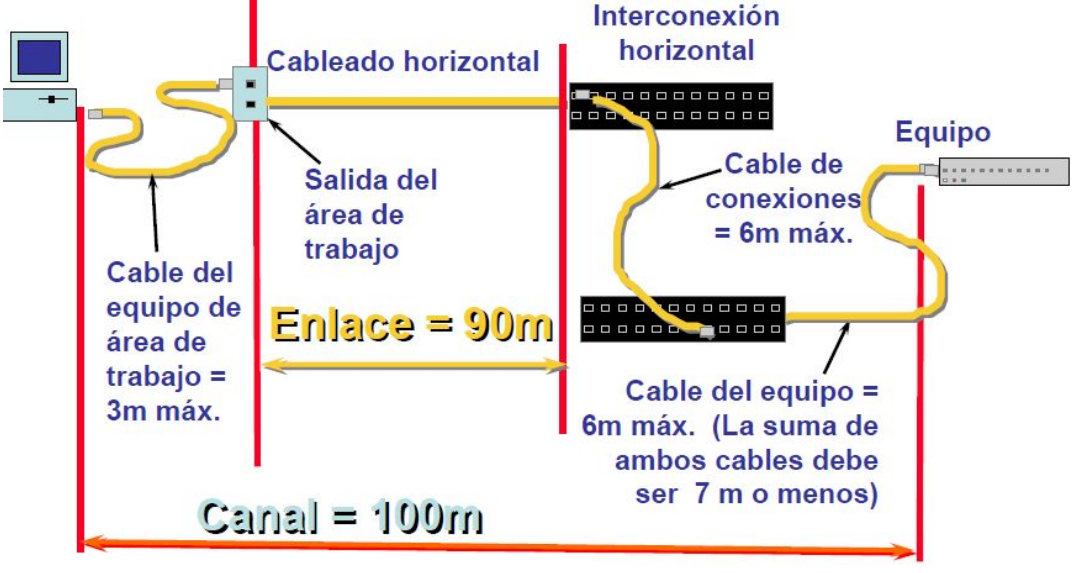
\includegraphics[width=.9\linewidth]{./media/distancias-maximas.png}
\end{center}
\subsection{Limitaciones}
\label{sec:org511fccd}
Evitar el paso de los cables de datos a través o cerca de:
\begin{itemize}
\item Motores eléctricos o transformadores. > 1,2m.
\item No compartir conducto con los cables de corriente alterna.
\item Fluorescentes a una distancia mínima de 12cm.
\item En caso de necesitar cruzar con cables eléctricos o luces fluorescentes, se debe hacer con un ángulo de 90º.
\item Equipos de soldadura, aires acondicionados, ventiladores, calentadores eléctricos a 1,2m
\item Evitar otras fuentes de radiofrecuencia o eléctricas
\end{itemize}
\section{Comprobación del cableado}
\label{sec:orgcf00c4e}
\subsection{Buenas prácticas}
\label{sec:org51353b7}
\begin{itemize}
\item Conviene ejecutar \emph{tests} conforme se avanza en la instalación.
\item Una vez finalizada la instalación, se debe ejecutar una prueba de conformidad o certificación
\end{itemize}
\subsection{Tareas a realizar}
\label{sec:orga4c4824}
\begin{itemize}
\item Verificar continuidad en los cables.
\item Verificar la calidad de la transmisión: niveles de diafonía, atenuación y ruido.
\item Chequear el mapeado de hilos: comprueba que los hilos que forman el cable estén montados correctamente.
\item Medir la resistencia del cable. Un valor alto puede producir problemas de atenuación de la señal
\item Longitud: distancia entre los dos extremos del cable. Tienen que respetar las distancias máximas definida por el estándar.
\end{itemize}
\end{document}
